\documentclass{article}

\usepackage{tikz}
\usepackage{amsmath}
\pagestyle{empty}

\begin{document}
\thispagestyle{empty}
\begin{picture}(0,0)
\put(0,-100){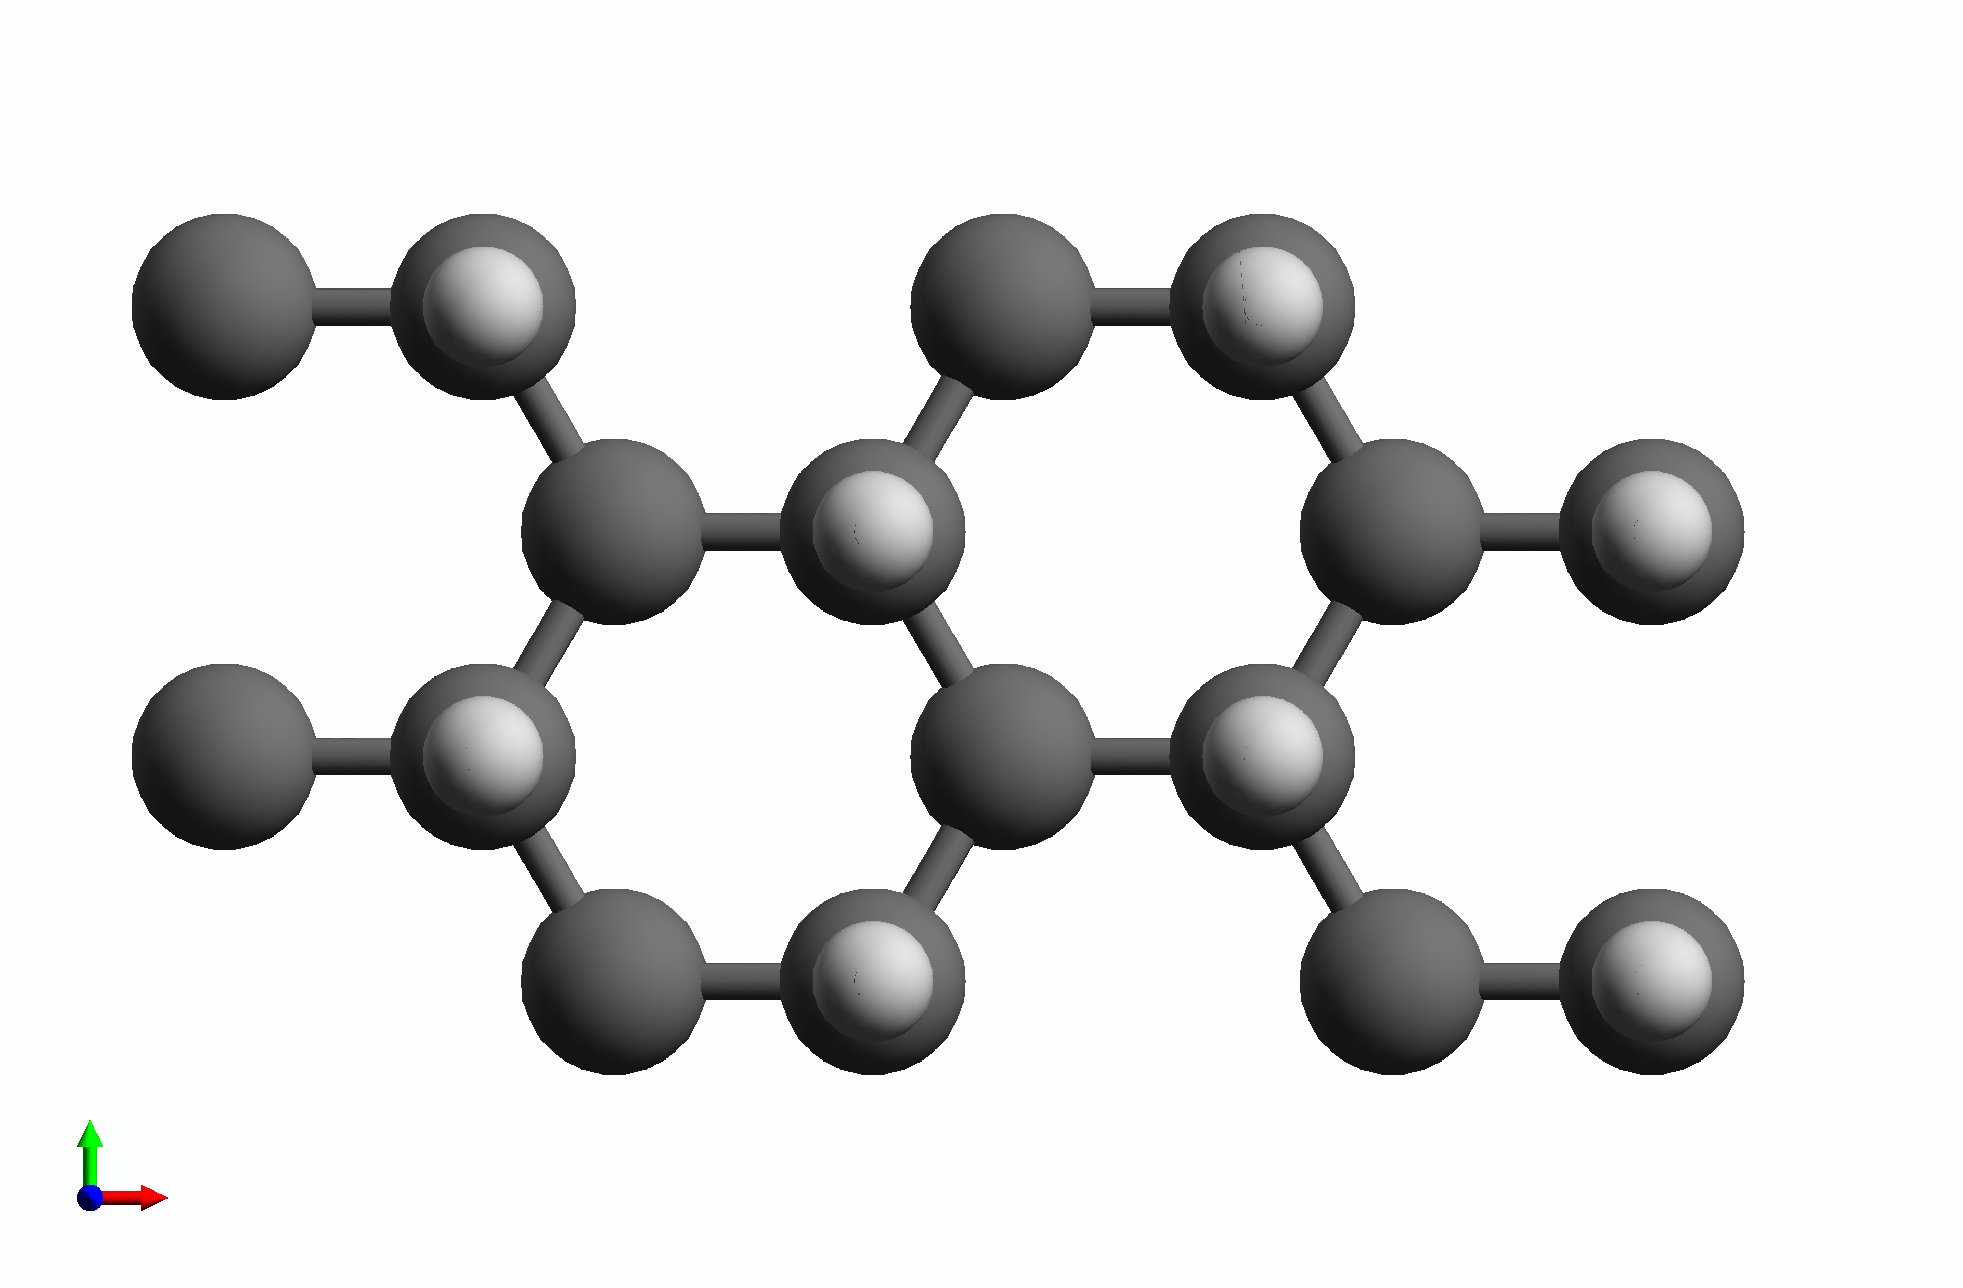
\includegraphics[width=0.8\textwidth]{up-1}}
\put(0,-100){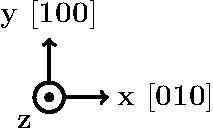
\includegraphics[width=0.2\textwidth]{arrows1}}

% \put(50,-15){\large{\textbf{1}}}
% \put(105,-45){\large{\textbf{1}}}
\put(66,-28){\large{\textbf{1}}}
\put(121,-60){\large{\textbf{1}}}
\put(7,-29){\large{\textbf{2}}}
\put(85,-29){\large{\textbf{2}}}
\put(60,-61){\large{\textbf{2}}}
\put(140,-61){\large{\textbf{2}}}

\end{picture}
\end{document}
